\section{SOFTWARE COMO SERVIÇO} 

A ideia de software como serviço é bastante difundida atualmente. 
Redes sociais, serviços de busca, serviços de \emph{streaming} de vídeo, são amplamente usados por todos. 
Segundo \citeonline{Fox2012} software como serviço, é definido como o software que entrega software e dados como serviços sobre a \emph{Internet}, usualmente via um programa como um \emph{browser} que roda num dispositivo cliente local, em detrimento de código binário que precisa ser instalado e que roda totalmente no dispositivo.

Várias vantagens são citadas em \citeonline{Fox2012}, tanto para usuários quanto para desenvolvedores de software. São elas:

\begin{enumerate}
	\item Desde de que os usuários não necessitam instalar a aplicação, eles não precisam se preocupar se possuem um hardware específico, ou se possuem uma versão específica de sistema operacional;
	\item Como os dados associados ao serviço geralmente são mantidos com o serviço, os usuários não precisam fazer \emph{bakcups}, nem se preocupar em os perderem devido a mal funcionamento, ou até mesmo os perderem devido a extravios;
	\item Quando um grupo de usuários querem coletivamente interagir sobre os mesmos dados, software como serviço é um veículo natural;
	\item Faz mais sentido manter grandes quantidades de dados centralizados e manter o acesso remoto a estes;
	\item Os desenvolvedores podem controlar as versões de software e sistema operacional que executam o serviço. Isto evita problemas de compatibilidade com distribuição do software devido ao grande número de plataformas que os usuários possuem. Além disso, é possível que o desenvolvedor teste novas versões do software usando uma pequena fração dos usuários temporariamente, sem causar distúrbios na maioria dos usuários;
	\item Como os desenvolvedores controlam a versão de execução do software, eles podem mudar até mesmo a plataforma dos mesmos, desde que não violem as \emph{Aplication Program Interfaces (APIs)} de interface com o usuário.
\end{enumerate}

	Para quem duvida do poder do software como serviço, é só observar que produtos consagrado como o \emph{Microsoft Office} já possuem versão como serviço, no caso o \emph{Microsoft Office 365}. Outros exemplos seriam o \emph{Twitter}, \emph{Facebook}, entre outros.
	

Segundo \citeonline{Fox2012}, na visão de mais alto nível, de cima para baixo na figura \ref{saas_view}, vê-se o software como um site na \emph{web}. 
O cliente acessa o servidor via \emph{internet} usando um \emph{browser HTML}. 
Na segunda visão, vê-se uma aplicação \emph{web} em três camadas, apresentação, lógica e persistência.
A camada de apresentação serve páginas \emph{HTML} para o usuário. Estas páginas consomem a camada lógica, também conhecida como camada de negócios, que são responsáveis pela lógica de negócio da aplicação. Por último vem a camada de persistência responsável pelo armazenamento e recuperação dos dados da aplicação.
A próxima visão é uma extensão da segunda, nela detalha-se mais a camada lógica, que internamente funciona com uma arquitetura \emph{model-view-controller}. 
Basicamente esta arquitetura define entidades de negócio (\emph{model}), que são manipuladas por controladores (\emph{controller}) e preparadas para apresentação pelo mecanismo de apresentação (\emph{view}).
A última camada corresponde as tecnologias e padrões de projetos adotados pela aplicação em sim. Por exemplo, na figura seleciona-se o padrão de projeto \emph{active record} para implementação do \emph{model},  usando o estilo arquitetural \emph{REST} para implementação do \emph{controller} e o padrão de projeto \emph{template view} para a implementação do \emph{view}. Estas escolhas são dependentes de projeto e geralmente são feitas por um arquiteto de \emph{software} experiente. 

\begin{figure}[ht]
	\centering
	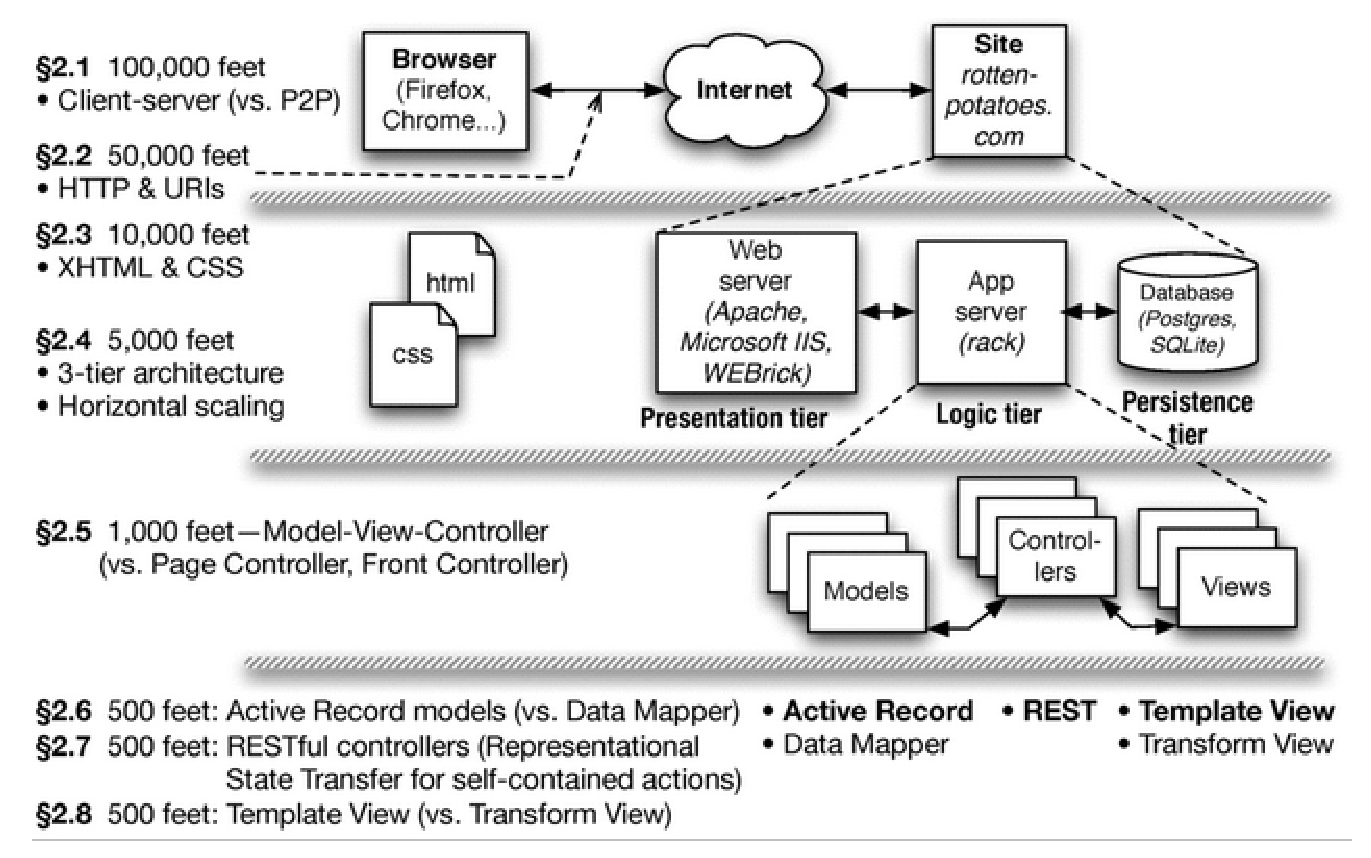
\includegraphics[width=15 cm]{figuras/saas_view.eps}
	\caption{Visões arquiteturais de software como serviço. Fonte: \citeonline{Fox2012}.}
    	\label{saas_view}
\end{figure}


